\begin{figure}
    \centering

    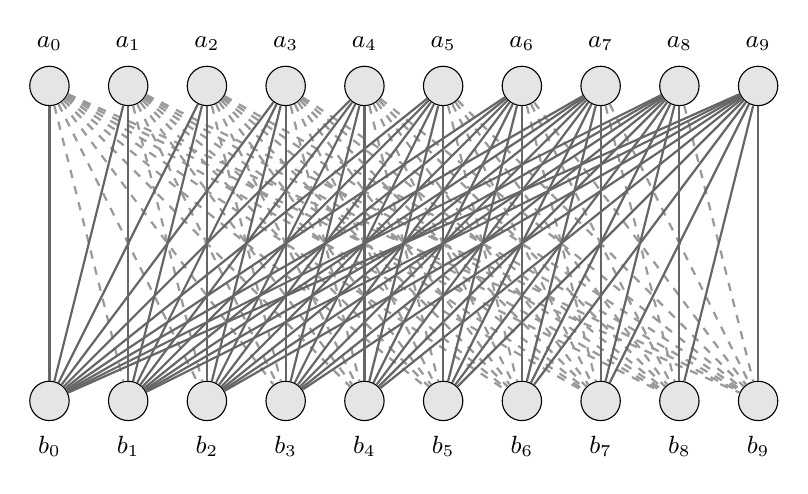
\begin{tikzpicture}[
        vertex/.style={circle, draw, fill=gray!20, minimum size=5mm, inner sep=1pt},
        label_a/.style={above=2pt, font=\small},
        label_b/.style={below=2pt, font=\small},
        node distance=1.5cm,
        solid edge/.style={draw, thick, black!60},
        dashed edge/.style={draw, dashed, thick, black!40},
        matrix cell/.style={draw, minimum size=0.5 cm, inner sep=0pt},
        matrix label/.style={font=\small, anchor=center}
    ]
	\node[vertex] (a_0) at (0,0) {};
	\node[vertex] (b_0) at (0,-4) {};
	\node[vertex] (a_1) at (1,0) {};
	\node[vertex] (b_1) at (1,-4) {};
	\node[vertex] (a_2) at (2,0) {};
	\node[vertex] (b_2) at (2,-4) {};
	\node[vertex] (a_3) at (3,0) {};
	\node[vertex] (b_3) at (3,-4) {};
	\node[vertex] (a_4) at (4,0) {};
	\node[vertex] (b_4) at (4,-4) {};
	\node[vertex] (a_5) at (5,0) {};
	\node[vertex] (b_5) at (5,-4) {};
	\node[vertex] (a_6) at (6,0) {};
	\node[vertex] (b_6) at (6,-4) {};
	\node[vertex] (a_7) at (7,0) {};
	\node[vertex] (b_7) at (7,-4) {};
	\node[vertex] (a_8) at (8,0) {};
	\node[vertex] (b_8) at (8,-4) {};
	\node[vertex] (a_9) at (9,0) {};
	\node[vertex] (b_9) at (9,-4) {};
	\draw[solid edge] (a_0) -- (b_0);
	\draw[dashed edge] (a_0) -- (b_1);
	\draw[dashed edge] (a_0) -- (b_2);
	\draw[dashed edge] (a_0) -- (b_3);
	\draw[dashed edge] (a_0) -- (b_4);
	\draw[dashed edge] (a_0) -- (b_5);
	\draw[dashed edge] (a_0) -- (b_6);
	\draw[dashed edge] (a_0) -- (b_7);
	\draw[dashed edge] (a_0) -- (b_8);
	\draw[dashed edge] (a_0) -- (b_9);
	\draw[solid edge] (a_1) -- (b_0);
	\draw[solid edge] (a_1) -- (b_1);
	\draw[dashed edge] (a_1) -- (b_2);
	\draw[dashed edge] (a_1) -- (b_3);
	\draw[dashed edge] (a_1) -- (b_4);
	\draw[dashed edge] (a_1) -- (b_5);
	\draw[dashed edge] (a_1) -- (b_6);
	\draw[dashed edge] (a_1) -- (b_7);
	\draw[dashed edge] (a_1) -- (b_8);
	\draw[dashed edge] (a_1) -- (b_9);
	\draw[solid edge] (a_2) -- (b_0);
	\draw[solid edge] (a_2) -- (b_1);
	\draw[solid edge] (a_2) -- (b_2);
	\draw[dashed edge] (a_2) -- (b_3);
	\draw[dashed edge] (a_2) -- (b_4);
	\draw[dashed edge] (a_2) -- (b_5);
	\draw[dashed edge] (a_2) -- (b_6);
	\draw[dashed edge] (a_2) -- (b_7);
	\draw[dashed edge] (a_2) -- (b_8);
	\draw[dashed edge] (a_2) -- (b_9);
	\draw[solid edge] (a_3) -- (b_0);
	\draw[solid edge] (a_3) -- (b_1);
	\draw[solid edge] (a_3) -- (b_2);
	\draw[solid edge] (a_3) -- (b_3);
	\draw[dashed edge] (a_3) -- (b_4);
	\draw[dashed edge] (a_3) -- (b_5);
	\draw[dashed edge] (a_3) -- (b_6);
	\draw[dashed edge] (a_3) -- (b_7);
	\draw[dashed edge] (a_3) -- (b_8);
	\draw[dashed edge] (a_3) -- (b_9);
	\draw[solid edge] (a_4) -- (b_0);
	\draw[solid edge] (a_4) -- (b_1);
	\draw[solid edge] (a_4) -- (b_2);
	\draw[solid edge] (a_4) -- (b_3);
	\draw[solid edge] (a_4) -- (b_4);
	\draw[dashed edge] (a_4) -- (b_5);
	\draw[dashed edge] (a_4) -- (b_6);
	\draw[dashed edge] (a_4) -- (b_7);
	\draw[dashed edge] (a_4) -- (b_8);
	\draw[dashed edge] (a_4) -- (b_9);
	\draw[solid edge] (a_5) -- (b_0);
	\draw[solid edge] (a_5) -- (b_1);
	\draw[solid edge] (a_5) -- (b_2);
	\draw[solid edge] (a_5) -- (b_3);
	\draw[solid edge] (a_5) -- (b_4);
	\draw[solid edge] (a_5) -- (b_5);
	\draw[dashed edge] (a_5) -- (b_6);
	\draw[dashed edge] (a_5) -- (b_7);
	\draw[dashed edge] (a_5) -- (b_8);
	\draw[dashed edge] (a_5) -- (b_9);
	\draw[solid edge] (a_6) -- (b_0);
	\draw[solid edge] (a_6) -- (b_1);
	\draw[solid edge] (a_6) -- (b_2);
	\draw[solid edge] (a_6) -- (b_3);
	\draw[solid edge] (a_6) -- (b_4);
	\draw[solid edge] (a_6) -- (b_5);
	\draw[solid edge] (a_6) -- (b_6);
	\draw[dashed edge] (a_6) -- (b_7);
	\draw[dashed edge] (a_6) -- (b_8);
	\draw[dashed edge] (a_6) -- (b_9);
	\draw[solid edge] (a_7) -- (b_0);
	\draw[solid edge] (a_7) -- (b_1);
	\draw[solid edge] (a_7) -- (b_2);
	\draw[solid edge] (a_7) -- (b_3);
	\draw[solid edge] (a_7) -- (b_4);
	\draw[solid edge] (a_7) -- (b_5);
	\draw[solid edge] (a_7) -- (b_6);
	\draw[solid edge] (a_7) -- (b_7);
	\draw[dashed edge] (a_7) -- (b_8);
	\draw[dashed edge] (a_7) -- (b_9);
	\draw[solid edge] (a_8) -- (b_0);
	\draw[solid edge] (a_8) -- (b_1);
	\draw[solid edge] (a_8) -- (b_2);
	\draw[solid edge] (a_8) -- (b_3);
	\draw[solid edge] (a_8) -- (b_4);
	\draw[solid edge] (a_8) -- (b_5);
	\draw[solid edge] (a_8) -- (b_6);
	\draw[solid edge] (a_8) -- (b_7);
	\draw[solid edge] (a_8) -- (b_8);
	\draw[dashed edge] (a_8) -- (b_9);
	\draw[solid edge] (a_9) -- (b_0);
	\draw[solid edge] (a_9) -- (b_1);
	\draw[solid edge] (a_9) -- (b_2);
	\draw[solid edge] (a_9) -- (b_3);
	\draw[solid edge] (a_9) -- (b_4);
	\draw[solid edge] (a_9) -- (b_5);
	\draw[solid edge] (a_9) -- (b_6);
	\draw[solid edge] (a_9) -- (b_7);
	\draw[solid edge] (a_9) -- (b_8);
	\draw[solid edge] (a_9) -- (b_9);
	\node[label_a] at (a_0.north) {$a_0$};
	\node[label_b] at (b_0.south) {$b_0$};
	\node[label_a] at (a_1.north) {$a_1$};
	\node[label_b] at (b_1.south) {$b_1$};
	\node[label_a] at (a_2.north) {$a_2$};
	\node[label_b] at (b_2.south) {$b_2$};
	\node[label_a] at (a_3.north) {$a_3$};
	\node[label_b] at (b_3.south) {$b_3$};
	\node[label_a] at (a_4.north) {$a_4$};
	\node[label_b] at (b_4.south) {$b_4$};
	\node[label_a] at (a_5.north) {$a_5$};
	\node[label_b] at (b_5.south) {$b_5$};
	\node[label_a] at (a_6.north) {$a_6$};
	\node[label_b] at (b_6.south) {$b_6$};
	\node[label_a] at (a_7.north) {$a_7$};
	\node[label_b] at (b_7.south) {$b_7$};
	\node[label_a] at (a_8.north) {$a_8$};
	\node[label_b] at (b_8.south) {$b_8$};
	\node[label_a] at (a_9.north) {$a_9$};
	\node[label_b] at (b_9.south) {$b_9$};
    \end{tikzpicture}
    \caption{A half-graph with 2 × 10 vertices. 
\emph{On the left}, solid lines show adjacent vertices, and dashed lines show non-adjacent vertices. 
Pairs of vertices without a line may or may not be connected. 
\emph{On the right} is the corresponding adjacency matrix.}
    \label{fig:test_half-graph}
\end{figure}
